\documentclass[12pt,twoside, a4paper, twocolumn]{article}
\usepackage[utf8]{inputenc}
\usepackage[brazil]{babel}
\usepackage[margin = 0.5in]{geometry}
\usepackage{amsmath}
\usepackage{amsthm}
\usepackage{amssymb}
\usepackage{amsthm}
\usepackage{setspace}
\usepackage[americanvoltages,fulldiodes,siunitx]{circuitikz}
\usepackage{lipsum}
\usepackage{pgfplots}
\usepackage{ifthen}
\usepackage{adjustbox}
\usepackage[section]{placeins}
\usepackage{hyperref}
\usepackage{graphicx}
\usepackage{adjustbox}
\pgfplotsset{compat=newest}
\graphicspath{ {./images/} }
%  #1 color - optional #2 x_0 #3 y_0 #4 x_f #5 y_f #6 name - optional  #7 true if adding lines to axis
\newcommand{\drawvector} [9] [color=cyan] {
\draw[line width=1.5pt,#1,-stealth](axis cs: #2, #3)--(axis cs: #4, #5) node[anchor=south west]{$#6$};
\ifthenelse{\equal{#7}{true}}{
\draw[line width=1pt,#1, dashed](axis cs: #4, #5)--(axis cs: #4, 0) node[anchor= north west]{$#8$};
\draw[line width=1pt,#1, dashed](axis cs: #4, #5)--(axis cs: 0, #5) node[anchor=south east]{$#9$};
}
{}
}
\newcommand\deriv[2]{\frac{\mathrm d #1}{\mathrm d #2}}
\title{Décimo Primeiro Relatório de Física Experimental 2}
\author{Henrique da Silva \\ hpsilva@proton.me}
\date{\today}
\pgfplotsset{width = 10cm, compat = 1.9}
\begin{document}
\maketitle
\pagenumbering{gobble}
\newpage
%pagenumbering{roman}
\tableofcontents
\newpage

\section{Introdução}

\paragraph*{Neste relatório, como utilizar difracao para fazer analise spectral de certos atomos, e tambem como utilizar um interferometro de Michelson para interpretar a interferncia da luz sob ela mesma.}

\paragraph*{Todos arquivos utilizados para criar este relatório, é o relatório em si estão em:  \url{https://github.com/Shapis/ufpe_ee/tree/main/4th semester/}}


\section{Analise spectral de gases}

\paragraph*{Primeiro vamos medir a lampada de helio, tabelar seus dados e achar um fator de correcao entre os dados medidos e os dados esperados.}

\subsection{Tabela de dados inicial}



\begin{center}
  \begin{tabular}{ |c|c|c| }
    \hline
    $\lambda \, medido$ & $\lambda \, real$ \\
    $(458 \pm 5)nm$     & $447nm$           \\
    $(479 \pm 5)nm$     & $470nm$           \\
    $(495 \pm 5)nm$     & $492nm$           \\
    $(503 \pm 5)nm$     & $502nm$           \\
    $(572 \pm 5)nm$     & $588nm$           \\
    $(639 \pm 5)nm$     & $668nm$           \\
    $(670 \pm 5)nm$     & $707nm$           \\
    \hline
  \end{tabular}
\end{center}

\subsection{Fator de correcao}
\begin{adjustbox}{scale=0.70}
  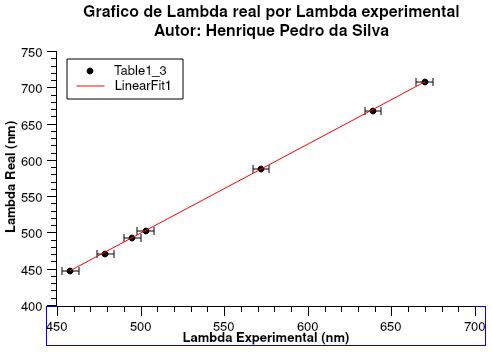
\includegraphics{Graph1.png}
\end{adjustbox}

\subparagraph*{Ajustando uma reta aos dados, temos:}

\begin{equation}
  \lambda_{real} = (1.230 \pm 0.006) \lambda_{exp} - (117.1 \pm 3.5)
\end{equation}

\subsection{Constante de Rydberg}

\paragraph*{Conseguimos observar tres linhas para o Hidrogenio ao inves das quatro esperadas. Isto ocorre porque duas das linhas esperadas na faixa do azul estao muito proximas.}

\paragraph*{Abaixo teremos a tabela de valores encontrados, e a direita, os valores "reais" encontrados ajustados pela equacao (1).}

\subsection{Tabela de Dados}

\begin{center}
  \begin{tabular}{ |c|c|c| }
    \hline
    $\lambda \, medido$ & $\lambda \, real$ \\
    $(446 \pm 5)nm$     & $(432 \pm 8)nm$   \\
    $(489 \pm 5)nm$     & $(484 \pm 8)nm$   \\
    $(631 \pm 5)nm$     & $(659 \pm 8) nm$  \\
    \hline
  \end{tabular}
\end{center}

\subsection{Achando R}

\begin{equation}
  R = \frac{1}{\lambda * \left(\frac{1}{n_f^2} - \frac{1}{n_i^2}\right)}
\end{equation}

\subparagraph*{Entao para nossos tres lambdas medidos teremos:}

\begin{equation}
  \begin{aligned}
     & \lambda = 432 \rightarrow R = 0.0110229276896 \\
     & \lambda = 484 \rightarrow R = 0.01101928374   \\
     & \lambda = 659 \rightarrow R = 0.01092564491   \\
     & R_{medio} = 0.01098928544                     \\
     & \varDelta R = 2.02727201e-9 = 0.000000002
  \end{aligned}
\end{equation}

\begin{equation}
  R = (0.010989285 \pm 0.000000002)nm^{-1}
\end{equation}

\paragraph*{Que esta bem proximo do valor esperado.}

\subsection{Motivo das linhas espectrais}

\subparagraph*{Os niveis de energia dos eletrons no atomo sao quantizados. Entao na sua transicao ele so pode emitir comprimentos de onda especificos dependendo da diferenca entre os niveis de energia que o eletron transitou.}

\subparagraph*{Ja no caso do corpo negro. As emissoes e absorcoes de energia sao ainda discretas, porem as projecoes dessas emissoes em relacao ao observador geram essa ilusao das ondas serem continuas, ja que para um numero arbitrariamente grande de particulas, as particulas seriam ejetadas em um numero arbitrariamente grande de direcoes.}

\subparagraph*{Pra ser honesto, no caso do corpo negro nao entendi bem. Eu tirei essa ideia daqui: \url{https://physics.stackexchange.com/questions/425127/black-body-radiation-and-spectra-lines}}

\section{O interferometro de Michelson}

\subsection{Medicoes}

\paragraph*{Apos varias medicoes, conseguimos que o $T_{m} = (12.2 \pm 0.5)mm$ que implica em $T_{m2} = (1.22 \pm 0.05)mm$}





\end{document}